%\documentclass[times]{MGS_class}
%%-----
%%Title und Author angeben
%\title{Style Guide}
%\author{Sebastian Szuzskiewicz and Sascha Kalab}
%%die Institute weiter unten zu den zugehörigen superscripts angeben
%
%\begin{document}
%
%\twocolumn[{\csname @twocolumnfalse\endcsname
%\begin{center}
%\maketitle
%%\thispagestyle{empty}
%
%%------
%%ANGABE DER INSTITUTE ANFANG
%
%\noindent \scriptsize \textsuperscript{1}\textsl{FH Technikum Wien, Game Engineering und Simulation, Wien, AUT}\\
%
%%ANGABE DER INSTITUTE ENDE
%%------
%\end{center}
%%\normalsize
%\hspace{15mm}
%
%}]%---

\begin{keywords}
Style, C++, Clean Code, Naming Conventions
\end{keywords}

\section{Why Style Guides} \label{sec:Introduction}%ein Sternderl (engl. asterisk) \section*{Einleitung} unterdrückt die Nummerierung der Überschriften, dann werden sie in Adobe Reader aber auch nicht im Strukturbaum angezeigt



A style guide is a set of standards for the writing and design of documents, either for general use or for a specific publication, organization, or field. A style guide establishes and enforces style to improve communication.

In the case of Computer Science, style guides help programmers to communicate with each other. If someone wants to use a specific library or function for example they need to understand what they want to include in their project. To accomplish this, style guides give programmers directive they can use to unify code.

But why do we want to do that? 

An example story from Robert C. Martins:
I know of one company that, in the late 80s, wrote a killer app. It was very popular, and lots of professionals bought and used it. But then the release cycles began to stretch. Bugs were not repaired from one release to the next. Load times grew and crashes increased. I remember the day I shut the product down in frustration and never used it again. The company went out of business a short time after that. Two decades later I met one of the early employees of that company and asked him what had happened. The answer confirmed my fears. They had rushed the product to market and had made a huge mess in the code. As they added more and more features, the code got worse and worse until they simply could not manage it any longer. It was the bad code that brought the company down. \citep{Martin-Code-2008}
This story shows that just bad written code brought down a company with huge potential. So the conclusion why code styles and style guides are needed is not only they help to communicate with other programmers but also you can spare time producing and maintaining code just with a good structured code style and codebase where everyone knows how to read through it.

\begin{figure}[!htbp] 
	\centering
	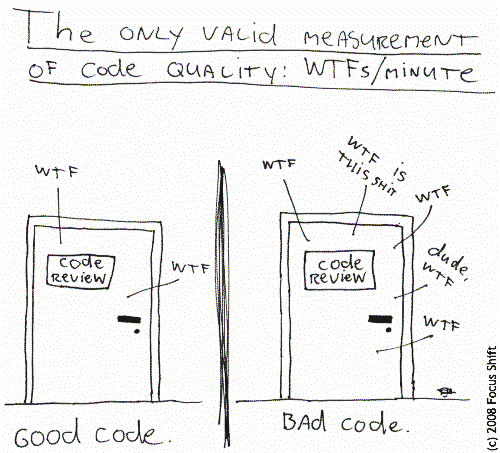
\includegraphics[width=0.7\columnwidth]{img/wtfcode.png}
	\label{fig:CodeMeasurement}
	\caption{\url{http://www.osnews.com/images/comics/wtfm.jpg}}
\end{figure}

As part of writing good code it has to be kept clean over time. Starting with the best intentions and messing up over periods of time still releases bad code. In order to accomplish this the coding style has to be used and respected all the time.

\section{Clean Code Style}
\subsection{Meaningful Names}
Programmers name various kinds of things like variables, functions or arguments. Naming is a huge part of good code, because every programmer has to do so much of it and because of that they should do it well.
\subsection{Intention-Revealing Names}
Choosing good names takes time but saves more than it takes. The name of a variable, function, or class, should answer all the big questions. It should tell you why it exists, what it does, and how it is used. If a name requires a comment, then the name does not reveal its intent.
\begin{lstlisting}[label={list:first}]
int d; // elapsed time in days
\end{lstlisting}
The name d reveals nothing. It does not evoke a sense of elapsed time, nor of days. Names should be chosen to specify what is being measured and the unit of that measurement:
\begin{lstlisting}[label={list:first}]
int elapsedTimeInDays;
int daysSinceCreation;
int daysSinceModification;
int fileAgeInDays;
\end{lstlisting}

\subsection{Avoiding Disinformation}
Programmers must avoid leaving false clues that obscure the meaning of code. Words whose entrenched meanings vary from our intended meaning should be avoided. For example, hp, aix, and sco would be poor variable names because they are the names of UNIX platforms or variants. Even if hypotenuse and hp looks like a good abbreviation for hypotenuse, it could be disinformative. \citep{Martin-Code-2008}

Refering to a grouping of accounts as an accountList is misinforming unless it is actually a List. The word list means something specific to programmers. If the container holding the accounts is not actually a List, it may lead to false conclusions. So accountGroup or bunchOfAccounts or just plain accounts would be better. \citep{Martin-Code-2008}

Using names which vary in small ways can also conclude in wrong information. How long does it take to spot the subtle difference between a XYZControllerForEfficientHandlingOfStrings in one module and, somewhere a little more distant, XYZControllerForEfficientStorageOfStrings? The words have frightfully similar shapes. \citep{Martin-Code-2008}

\subsection{Pronounceable Names}
Humans are good at words. A significant part of brains is dedicated to the concept of words. And words are, by definition, pronounceable. It would be a shame not to take advantage of that huge portion of our brains that has evolved to deal with spoken language. So make your names pronounceable. \citep{Martin-Code-2008}
Example from Robert C. Martins:
A company I know has genymdhms (generation date, year, month, day, hour, minute, and second) so they walked around saying “gen why emm dee aich emm ess”. I have an annoying habit of pronouncing everything as written, so I started saying “gen-yah-muddahims.” It later was being called this by a host of designers and analysts, and we still sounded silly. But we were in on the joke, so it was fun. Fun or not, we were tolerating poor naming. New developers had to have the variables explained to them, and then they spoke about it in silly made-up words instead of using proper English terms. Compare
\begin{lstlisting}[label={list:first}]
class DtaRcrd102
{
    private Date genymdhms;
    private Date modymdhms;
    private final String pszqint = "102";
    /* ... */
};

to

class Customer
{
    private Date generationTimestamp;
    private Date modificationTimestamp;;
    private final String recordId = "102";
    /* ... */
}; 
\end{lstlisting}

Intelligent conversation is now possible: “Hey, Mikey, take a look at this record! The generation timestamp is set to tomorrow’s date! How can that be?”

\subsection{Searchable Names}
Single-letter names and numeric constants have a particular problem in that they are not easy to locate across a body of text. 
One might easily grep for MAX\_CLASSES\_PER\_STUDENT, but the number 7 could be more troublesome. Searches may turn up the digit as part of file names, other constant definitions, and in various expressions where the value is used with different intent. It is even worse when a constant is a long number and someone might have transposed digits, thereby creating a bug while simultaneously evading the programmer's search. 
Likewise, the name e is a poor choice for any variable for which a programmer might need to search. It is the most common letter in the English language and likely to show up in every passage of text in every program. In this regard, longer names trump shorter names, and any searchable name trumps a constant in code. \citep{Martin-Code-2008}

\section{PascalCase and camelCase}
CamelCase is the practice of writing compound words or phrases such that each word or abbreviation begins with a capital letter. Camel case may start with a capital or, especially in programming languages, with a lowercase letter. Common examples are LibreOffice, PowerPoint, iPhone or in online usernames such as UserName.
In Microsoft documentation, camel case always starts with a lower case letter (e.g. backColor), and it is contrasted with PascalCase which always begins with a capital letter (e.g. BackColor).
The use of medial caps for compound identifiers is recommended by the coding style guidelines of many organizations or software projects. For some languages (such as Mesa, Pascal, Modula, Java and Microsoft's .NET) this practice is recommended by the language developers or by authoritative manuals and has therefore become part of the language's ''culture''.
Style guidelines often distinguish between upper and lower camel case, typically specifying which variety should be used for specific kinds of entities: variables, record fields, methods, procedures, types, etc. These rules are sometimes supported by static analysis tools that check source code for adherence.
The original Hungarian notation for programming, for example, specifies that a lowercase abbreviation for the ''usage type'' (not data type) should prefix all variable names, with the remainder of the name in upper camel case; as such it is a form of lower camel case.
Programming identifiers often need to contain acronyms and initialisms that are already in upper case, such as "old HTML file". By analogy with the title case rules, the natural camel case rendering would have the abbreviation all in upper case, namely ''oldHTMLFile''. However, this approach is problematic when two acronyms occur together (e.g., ''parse DBM XML'' would become ''parseDBMXML'') or when the standard mandates lower camel case but the name begins with an abbreviation (e.g. ''SQL server'' would become ''sQLServer''). For this reason, some programmers prefer to treat abbreviations as if they were lower case words and write ''oldHtmlFile'', ''parseDbmXml'' or ''sqlServer''.
A proper definition of the usage of Camel- and PascalCase is given in the following chapters.
\url{https://en.wikipedia.org/wiki/CamelCase}

\section{How to write comments}
Comments are an essential part of your code as they aid the reader in understanding it. This does not mean comments are a cure for poorly written code in terms of formatting, naming and style. They should be aimed to assist clarifying certain parts, e.g. complex operations or the meaning of hard coded integer values. Writing good comments is a bit of an art itself and the rule of thumb is ''Quality over quantity''.

The idea is to write as less comments as possible with the best result possible, meaning that code should be self-explanatory as far as the language allows to. Also, comments should explain the ''why'' rather than the ''what'' because the ability of reading code implicitly clarifies the “what” most of the time. Another important thing to keep in mind is that comments cannot replace code, so writing a comment that states a certain header file needs to be included or the value of a variable should be in a certain range is not a good habit. This is the responsibility of code and should not be in a comment.

At best a comment shortly describes something and does not distract the reader from the code. It is important to keep comments from being ambiguous and they need to always be updated when the code their assigned to is. The worst thing comments can do to a reader, which could be the author of a piece of code himself, is that they do not tell the truth anymore or just repeat what the code can say itself.

\section{Formatting}
Formatting makes code readable to the human eye. A compiler does not care about that since it only processes bytes of information. Keeping code in a nice and readable format is one of the most important things to do besides making it work correctly.
\begin{quote}
''You should take care that your code is nicely formatted. You should choose a set of simple rules that govern the format of your code, and then you should consistently apply those rules.'' \citep{Martin-Code-2008}
\end{quote}
Good and consistent formatting is more important than just getting code to work. It makes code more maintainable as well as extensible and helps keeping track of the big picture. When working in a team, tools should be used with common rulesets for all team members. Such tools and rulesets will be discussed in later sections.
Main parts of formatting are:
\begin{enumerate}
\item Indentation
\item Bracketing
\item Ordering of Sections
\item Placement of Blanks
\end{enumerate}

\subsection{Indentation}
Indentation is about horizontal placement of code and where a line starts. It helps in keeping track of which section a line of code belongs to and makes reading a lot easier. Wrong indentation is disastrous for reading and can easily lead to misunderstandings. Whether indentation is achieved through blanks or tabulators is not that important as to keep it consistent. Furthermore it is a matter of taste whether the body of a section should be indented or kept in the same vertical line as the beginning, e.g. the body of a switch-case statement.

\subsection{Bracketing}
There is a lot that could be said about setting brackets and what is too much. First of all, there is more to it than just where to set the opening bracket of a function or if-statement body. For example, most Java programmers prefer to place the opening bracket in the same line as the function header whereas most C\# programmers will set it in the next line.
Truth is, overusing of brackets can make code unreadable for humans but not for machines. Similar to comments the compiler has no problem resolving and respecting all used brackets as long as they are syntactically correct. A human on the other hand is easily overwhelmed even with a small number of brackets. Imagine the following line as an example:
\begin{lstlisting}[label={list:first}]
int a = (b + (c * d));
\end{lstlisting}
There is actually no need of any brackets at all in this line of code. The operator precedence will make sure that the compiler knows what to do in this case, still the brackets are not wrong syntactically. In some situations though, it is necessary to set brackets to ensure the wanted behaviour. As barley any programmer knows the exact order of the operator precedence table brackets are useful but they should be kept to a minimum.

\subsection{Ordering of Sections}
Ordering is actually not just about sections but also about functions. Functions should be grouped in a way so that is easy to find functions that belong and are used together. For sections it has the meaning of sections in a class header layout, if the programming language uses that concept. Member variables of a class should be grouped together as well as so called ''getter'' and ''setter'' functions. It is common practise to keep member variables either at the top or the bottom of a class definition. Either way, constructors and operators should be first followed by possible other functions.

\subsection{Placement of Blanks}
This topic is bit about nit-picking since it does not improve readability of code this much. Still it something to discuss as it is part of a formatting rule set. Besides a syntactic rules of the used language, blanks should be placed where it helps making the code more readable, e.g. to indicate operator precedence without using brackets. Generally it is ''Quality over quantity'' again.

\section{Don’ts of Code Style}
The following section describes some of the most done mistakes in code styling that affect readability and maintainability of code. Some of these ''Don'ts'' may have funny names but horrendous impacts.

\subsection{Yoda Conditions}
Seen in the code of some programmers the so called “Yoda Conditions”, which got their name from the famous Star Wars character, are over read easily but leave the feeling that something is wrong with the code. They appear when a programmer writes an if-statement and puts the constant before the variable:
\begin{lstlisting}[label={list:first}]
if (1 == myInt)
\end{lstlisting}
The correct way to do this is to simply put the variable before the constant which makes a lot more sense and prevents a possible read from scratching his head.

\subsection{Fake Comments}
When comments without any useful information are placed somewhere in code just with the purpose of silencing a tool like ''FxCop'' they are wrong. The right way is to actually give information about why a piece of code was written.

\subsection{Monolithic Functions and schizophrenic Classes}
Functions that are way too long and complex usually do too much work on their own. They are monolithic and combine logic which should actually be split up into several functions to make the code reusable, more readable and most important more maintainable.

The term ''schizophrenic class'' indicates that a class has more than one purpose which is plain wrong and should be avoided. One class has only one purpose and consequently ignoring this paradigm can lead to various problems with more or less impact on code quality.

\section{Code Style Guide Example for C++}
In the following a style guide for C++ code is presented. It is meant to be a guideline to keep in mind when writing code. These guidelines are mainly focused on C++ code in general but certain points (e.g. exception handling) address game related code. Further reading: \url{https://google.github.io/styleguide/cppguide.html}

\subsection{Naming Conventions}
\subsubsection{Classes / Interfaces / Base Classes}
Class names in general, as well as interfaces or base classes, should be written in PascalCase style and should be a noun or a combination of nouns.

Example: WindowController

Interfaces, which have the condition not to contain any members but functions, should start with the letter ''I'' followed by one or more nouns.

Example: IObserver

Base classes should be named like normal classes with the extension ''Base'' at the end.

Example: BehaviourBase

Naming classes in that scheme makes it obvious to other programmers what kind of class they are dealing with and how to use it. Additionally it makes searching for a specific type of class a lot easier.

\subsubsection{Variables}
Variables do not have a general rule applying to all of them. They have to be differentiated depending on the scope they exist in. Global scope is not listed below as global variables should be avoided but in case a global variable is necessary or of specific benefit it should be written in either PascalCase or camelCase and prefixed with ''g\_''.

Example: g\_Count

\textbf{Local Variables / Parameters}

Variables local to a function as well as parameter variables should be written in camelCase without any prefix at all.

Example: distanceToGoal

\textbf{Member Variables}

Variables in class scope (member variables) should be written in either PascalCase or camelCase but either way prefixed with ''m\_''.

Example: m\_Position – or – m\_orientation

\subsubsection{Functions}
Function names in general, independent of their scope, should simply be written in PascalCase and should usually consist of verbs.

Example: CalculateSteering

\textbf{Getter / Setter Functions}

So called ''Getter'' and ''Setter'' functions are used to get access to member variables that are not directly accessible. They should be named similar to the member variable they are assigned to but with the prefix ''Get'' or ''Set''. That way it is easy to see which data of a class can be retrieved and which can be set.

Example: GetPosition – or - SetOrientation

\subsubsection{Templates}
This section only applies to type template parameters. Since C++ allows two keywords to declare a type template parameter it should be differentiated between a parameter which is meant to be a simple type and a parameter which is meant to be a custom type. For simply types the template parameter should be declared using ''typename'' and for a complex type ''class'' should be used.

Example: template<typename T, class U> Select(…)

\subsection{General Rules}
\subsubsection{Include Guard}
Every header file has to have a so called ''include guard'' which usually is a pre-processor statement in the very first line(s). Most modern compilers support the ''\#pragma once'' command but for compatibility and standard conformity reasons an ''\#ifndef'' or ''\#if'' command should also be used. Notice that the last two command need to be closed at the very end of the header file placing a ''\#endif'' command.
Example:
\begin{lstlisting}[label={list:first}]
#pragma once
#ifndef HEADER_FILE_NAME_H_
<code>
#endif // HEADER_FILE_NAME_H_
\end{lstlisting}

\subsubsection{Exceptions}
In game related code exceptions are a bad practise and should not be used at all. The reason for that is they are slow and not very well implemented in C++.

\subsubsection{Bracket Placement}
In general brackets should be used even when they can be left out without creating syntactic errors. For example an if-statement with only on line in its scope. It makes code much more readable and avoids painful errors.

On the other hand parenthesis should not be overused but every time it supports readability. Common sense is helpful for this kind of brackets.

\section{CppCheck}
\subsection{Description}
Cppcheck is a static analysis tool for C/C++ code. Unlike C/C++ compilers and many other analysis tools it does not detect syntax errors in the code. Cppcheck primarily detects the types of bugs that the compilers normally do not detect. The goal is to detect only real errors in the code (i.e. have zero false positives).

\subsection{Integration in Development Tools}
Cppcheck is integrated with many popular development tools. For instance:
\begin{enumerate}
\item Clion - Cppcheck plugin
\item Code::Blocks - integrated
\item CodeDX (software assurance tool) - integrated
\item CodeLite - integrated
\item CppDepend 5 - integrated
\item Eclipse - Cppcheclipse
\item gedit - gedit plugin
\item Hudson - Cppcheck Plugin
\item Jenkins - Cppcheck Plugin
\item Mercurial (Linux) - pre-commit hook - Check for new errors on commit (requires interactive terminal)
\item Tortoise SVN - Adding a pre-commit hook script
\item Git (Linux) - pre-commit hook - Check for errors in files going into commit (requires interactive terminal)
\item Visual Studio - Visual Studio plugin
\end{enumerate}

\subsection{Features}
\begin{enumerate}
\item Out of bounds checking
\item Memory leaks checking
\item Detect possible null pointer dereferences
\item Check for uninitialized variables
\item Check for invalid usage of STL
\item Checking exception safety
\item Warn if obsolete or unsafe functions are used
\item Warn about unused or redundant code
\item Detect various suspicious code indicating bugs
\end{enumerate}

For a full description of all features look at: \url{http://sourceforge.net/p/cppcheck/wiki/ListOfChecks}
Both command line interface and graphical user interface are available.

\subsection{Usage}
As with many analysis programs, there are many unusual cases of programming idioms which may be acceptable in particular target cases, or outside of the programmer's scope for source code correction. A study conducted in March 2009 identified several areas where false positives were found by cppcheck, but did not specify the program version examined. Cppcheck has been identified for use in systems such as CERNs 4DSOFT meta analysis package, for code verification in high energy particle detector readout devices, system monitoring software for radio telescopes as well as in error analysis of large projects, such as OpenOffice.org and the Debian archive.

The idioms and terms, as described in this styleguide or from various other resources, need to be entered in cppcheck.

\subsection{Where to get from?}
Cppcheck can either be downloaded directly from: \url{http://sourceforge.net/projects/cppcheck/} or integrated in various development tools via specific options (see Features).

\subsection{Support}
The IRC channel can be access with a web browser: \url{http://webchat.freenode.net}
Forum: \url{http://sourceforge.net/p/cppcheck/discussion/}


% Bibliography



% Option 1: Bibliography generation with BibTeX:
% Add all refernces to the *.bib file (here Literatur.bib). Then run LaTeX, BibTeX, and again twice LaTeX.
% Use \cite{kop05} within the text for a citation.
% - GEMRAN ----------
%\bibliographystyle{apalike-url-de} %ermöglicht longnamesfirst Option. Bei erster Erwähnung werden alle Autoren gennannt in der Folge et al. verwenden wir aber nicht
% - END GERMAN-------
%% -ENGLISH---------

%\bibliographystyle{apalike-url-de}
%%% -END ENGLISH------
%\bibliography{Bibliography}
%% Option 2: Bibliography generation without BibTeX:
%%\begin{thebibliography}{99}
%%\bibitem[kop05]{kop05}
%%H.~Kopka, {\em LaTeX, Band 1: Einf"uhrung}, Pearson Studium, M"unchen, 3.~Auflage, 2005.
%%\bibitem[knu98]{knu98}
%%F.~Mittelbach, M.~Goossens, J.~Braams, D.~Carlisle, and Ch. Rowley, {\em The LaTeX Companion}, 
%%Addison-Wesley, 2nd edition, 2004.
%%\end{thebibliography}
%
%\end{document}